\documentclass[12pt,letterpaper,noanswers]{exam}
\usepackage[usenames,dvipsnames,svgnames,table]{xcolor}
\usepackage[margin=0.9in]{geometry}
\renewcommand{\familydefault}{\sfdefault}
\usepackage{multicol}
\pagestyle{head}
\definecolor{c03}{HTML}{FFDDDD}
\header{AM 108 Class 07}{}{bistability}
\runningheadrule
\headrule
\usepackage{graphicx} % more modern
\usepackage{amsmath} 
\usepackage{amssymb} 
\usepackage{hyperref}
\usepackage{tcolorbox}

\begin{document}
 \pdfpageheight 11in 
  \pdfpagewidth 8.5in

\noindent 
\begin{itemize}
\itemsep0em
    \item There is a Check Yourself pre-class assignment for Monday
    \item There is a two question skill check on Monday.  The sample questions for it are below.
    \item Before attending OH, post to \#officehours on Slack (or the Office Hours thread on Piazza) to let your classmates and the course staff know what questions / problems you're bringing to OH.
    \item OH this week: 3-4pm Friday.  Find the zoom links (and the person staffing the OH) on Canvas.
    \item OH next week: 10-11am ET Tuesday, 3-4pm and 7-8:30pm Wednesday, 4-5pm an 8-9:30pm Thursday, 3-4pm Friday.
    \end{itemize}

\hrule
\vspace{0.2cm}

\noindent\textbf{Teams}

\begin{multicols}{2}
1. 
\end{multicols}

\noindent \textbf{Teams 5 and 6}: Post screenshots of your work to the course Google Drive today.  Include words, labels, and other short notes that might make those solutions useful to you or your classmates.  Find the link in Canvas (or here: \url{https://drive.google.com/drive/u/0/folders/1GcpwvKHD4tMecpFQ4lNxN_r5Ylj7YHbd})

\vspace{0.2cm}
\hrule
\vspace{0.2cm}


\noindent \textbf{Extra vocabulary / extra facts:}
\begin{tcolorbox}
A \textbf{parameter space} is a space where each coordinate is a parameter.

A \textbf{bifurcation curve} is a curve in parameter space where, at every point along the curve, the associated parameter set is a bifurcation point (meaning that a bifurcation occurs in the system at that set of parameter values).

A \textbf{stability diagram} shows bifurcation curves plotted in parameter space.  The bifurcation curves split the parameter space into regions with qualitatively different phase portraits.

A \textbf{cusp bifurcation} is a type of bifurcation that can occur in a system with two parameters.  At the bifurcation point two branches of saddle-node bifurcation curves meet tangentially.  This bifurcation is sometimes referred to as a \textbf{cusp catastrophe}.

A \textbf{cusp catastrophe} surface is the surface of fixed points in (parameter,$x$)-space associated with a cusp bifurcation.  A plot in (parameter,$x$)-space is analogous to a bifurcation diagram (but we often don't indicate stability, and there is a second parameter so the plot is in 3-space).

\textbf{Hysteresis} is a history dependence in the state of the system.  The state of the system when at a particular set value may be different depending on the prior history of that state.  It often occurs in bistable systems.
\end{tcolorbox}


\vspace{0.2cm}

\hrule
\vspace{0.2cm}

\noindent\textbf{Example with a cusp bifurcation}

$\dot x = h + r x - x^3$

The bifurcation diagram are made for $r = -1.5, 0, 1.5, 3$.  You'll see that for $r<0$ there are no bifurcations in the system.  For $r > 0$ there are two saddle-node bifurcations.  These saddle-node bifurcations move apart as $r$ increases.

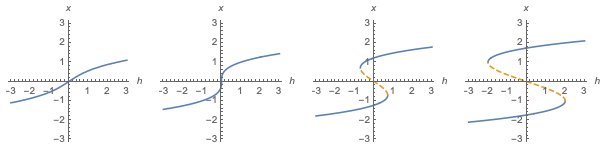
\includegraphics[width=0.9\linewidth]{img/C08stabilitybifn.png}

This stability diagram shows the location of the saddle-node bifurcations in $hr$-space.

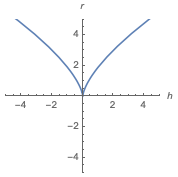
\includegraphics{img/C08stability.png}


\vspace{0.2cm}
\hrule
\vspace{0.2cm}


\noindent\textbf{Skill Check C08 practice}
\begin{questions}
\item (C05) Retake of the C05 skill check question.  This is the one where you add a cobweb to an $f(x)$ vs $x$ plot (where the $y = x$ line is on the plot as well).

\item 
Plot the function $f(N) = H\dfrac{N^2}{A^2+N^2}$.  

\emph{Label your axes and to include at least one (labeled) tick mark on each axis.}

Your plot should have correct behavior for $N\rightarrow 0$, for $N\rightarrow\infty$, and for an appropriate (and labeled) finite value of $N$.

\end{questions}




\vspace{0.2cm}

\hrule
\vspace{0.2cm}

\noindent\textbf{Skill Check C08 practice solution}

\begin{questions}
\question See C04 handout.
\question 

One way to think of this function is as $f(N) = H \dfrac{(N/A)^2}{1+(N/A)^2}$, where $N/A$ is dimensionless.  Let $ x = N/A$.  

The $N$-axis (horizontal) is naturally measured in increments of $A$.  The vertical in increments of $H$.  

As $x\rightarrow \infty$, we have $\lim_{x\rightarrow \infty} H \dfrac{x}{1+x} = H$.  At $x = N/A = 0$ we have $f(0) = H\frac{0}{1+0} = 0$.  At $x = 1$ so $N = A$ we have $f(A) = H\dfrac{A^2}{2A^2} = H/2$.  

The slope as $N\rightarrow 0$ is given by $\left.f'(x)\right\vert_0 = \left.H(2N)(A^2+N^2)^{-1}-HN^2(2N)(A^2+N^2)^{-2}\right\vert_{N=0} = 0$.  Or, using the binomial expansion to approximate the function near $0$, $f(N)= H(N/A)^2(1+(N/A)^2)^{-1} \approx H(N/A)^2(1 - (N/A)^2 + ...)$ (we have $N/A \ll 1$ when $N$ is close enough to $0$).  And for $N$ close to zero, this is $f(N) \approx HN^2/A^2$ (a parabola).

We're now ready to sketch.  The curve passes through $(0,0)$ and leaves the origin going horizontally (tangent to the $N$-axis).  Close to $0$, $f(N) \approx H \dfrac{N^2}{A^2}$, so it will specifically leave the origin with a parabolic shape.  It passes through $f(A) = H/2$ and approaches $H$ as $N \rightarrow\infty$.

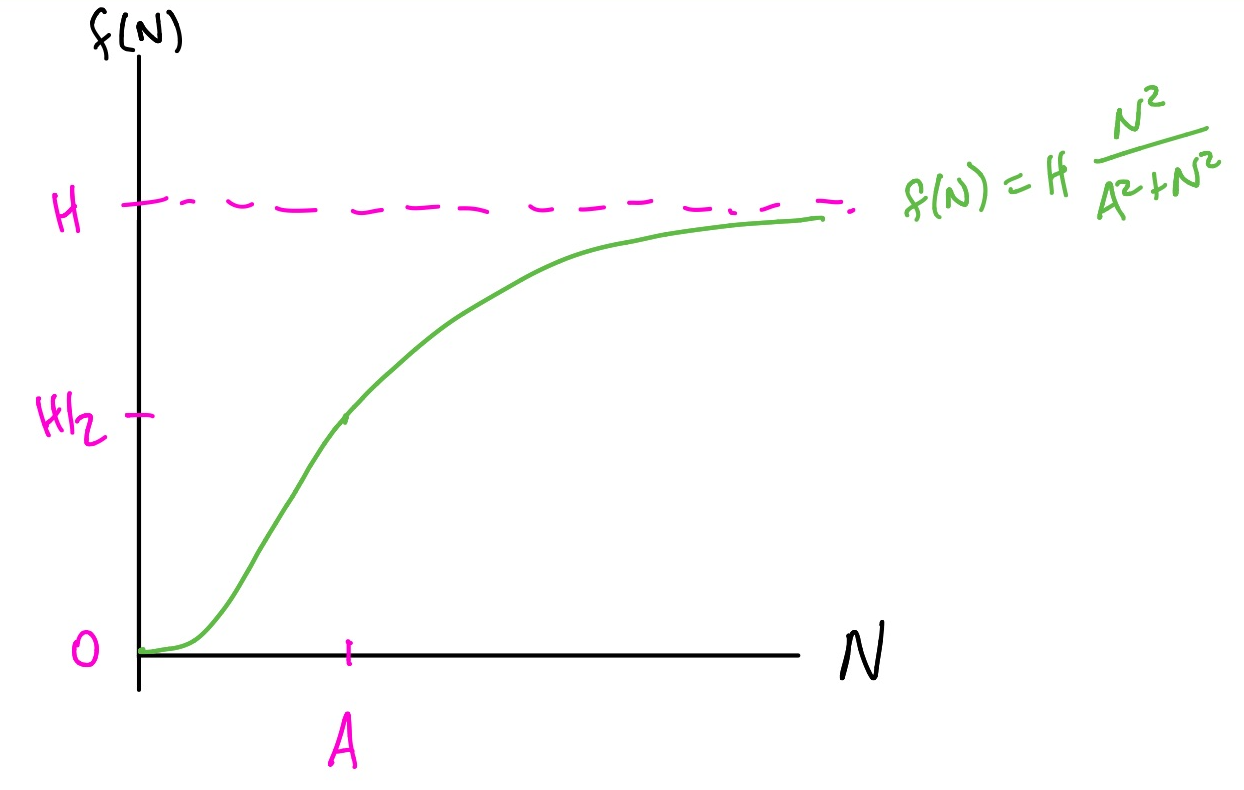
\includegraphics[width=3in]{img/C08soln-Hillfcnplot-p1.png}

\end{questions}

\vspace{0.2cm}

\hrule
\vspace{0.2cm}

\noindent\textbf{Questions}


In your post to the \#classactivities Slack channel, provide the number of the question you're posting about.

\begin{questions}
\item (4.3.3) For $\dot{\phi} = \mu \sin \phi - \sin 2\phi$:
\begin{parts}
\item (\textbf{Team 2}, post to slack about this if you get to this problem)

Check that the vector field is well-defined on the circle.
\item (\textbf{Team 5}, post to slack about this if you get to this problem)

Draw the qualitatively different phase portraits that exist at different values of $\mu$.
\item (\textbf{Team 6}, post to slack about this if you get to this problem)

Classify the bifurcations that occur as $\mu$ varies.
\item (\textbf{Team 7}, post to slack about this if you get to this problem)

Find the bifurcation values of $\mu$. 
\item (\textbf{Team 2}, post to slack about this if you get to this problem)

Think of $\phi$ as describing the \textbf{phase of a single oscillator}.  For what values of $\mu$ is the system ``oscillating''?
\item (\textbf{Team 5}, post to slack about this if you get to this problem)

Think of $\phi$ as describing the \textbf{phase difference} between an oscillator and a reference.  For what values of $\mu$ is the oscillator entrained (phase-locked) to the reference?
\end{parts}

\emph{You might use Mathematica to find or check the shapes of the bifurcation diagrams}

\item Consider the nondimensionalized fish population model $\dot x = x(1-x) - h$ where $h$ is a harvesting term.

In this model there is not a feedback between the population of fish ($x$) and the harvesting term ($h$). 
To identify the bifurcation structure of this system, sketch $x(1-x)$ and $h$ both vs $x$. 

\begin{parts}
    \item What kind of bifurcation occurs in this system?
    \item Let $h = h_c$ denote the bifurcation point.  At $h<h_c$ and $h>h_c$ what is the long term behavior?  (i.e. what is this model predicting for the fishery?)
\end{parts}   

\item In the model above, it was possible for the population to become negative because the harvesting rate did not respond to the fish population: ``harvesting'' continued in the model even when the fish were gone.

Consider $\dot x = x(1-x) - h\dfrac{x}{a+x}$.  This harvesting term has a feedback: the harvesting rate now depends on $x$.

\begin{parts}

\part Notice that $x=0$ is a fixed point of the system.  Identify its stability as a function of parameters.

\part Identify how many fixed points the system can have and find the qualititatively different phase portraits that exist at different parameter sets.
\emph{To think about other fixed points, one option is to follow the steps below}
\begin{itemize}
    \item Plot $1-x$ and $h\dfrac{1}{a+x}$.  \emph{Do this plotting via your own reasoning, rather than using a computational tool}.
    \item Consider how the shape of $h\dfrac{1}{a+x}$ depends on $a$ and on $h$.  Argue that the system could have one, two, or three fixed points
\end{itemize}  

\part How did making the harvesting rate depend on the state of the system change the model predictions?

\end{parts}

\end{questions}

\vfill

\eject
\noindent\textbf{Selected Answers}.

1a: $\mu\sin(\phi+2\pi) -\sin(2\phi+ 4\pi) = \mu\sin\phi-\sin 2\phi$.  well-defined.  1b: draw for $\mu$ very negative, zero, and very positive.  Then add in an in-between case.  1c: Two subcritical pitchfork bifurcations.  1d: $\mu\sin\phi$ is tangent to $\sin 2\phi$ at the $0$ fixed point when $\mu\phi$ (the linear approximation) is equal to $2\phi$, so when $\mu = 2$.  At $\pi$ the tangency occurs when $\mu = -2$.  So a subcritical pitchfork for $\phi = 0$ and $\mu = 2$ and a subcritical pitchfork for $\phi = \pi$ at $\mu = -2$.  1e: no oscillation ever.  1f: there is always entrainment (there is always a fixed point).

2:

3:
\end{document}